\newpage
\section{Problem 5.6}
对于$q(\bm{x})=(10x_1^2-18x_1x_2+10x_2^2)/2+4x_1-15x_2+13$

\subsection{重要参数}

\[G=\begin{bmatrix}
10&-9\\
-9&10
\end{bmatrix},\qquad \lambda_1=19,\lambda_2=1,\qquad (\dfrac {\lambda_{1}-\lambda_{2}}{\lambda_{1}+x_{2}})^2 =0.81\]

\subsection{算法伪代码}
\begin{algorithm}[h]  
\caption{Steepest-denscent method for problem(5.6)}  
\begin{algorithmic}[1]  
\STATE Given $\bm{x}^{(0)}$ and $G$
\STATE Set $\bm{p}^{(0)}=-\bm{g}^{(0)},k=0$
\WHILE {$\|\bm{g}^{(k)}\|>\epsilon$}
\STATE Set $\alpha_k=-\dfrac{{{\bm{p}^{(k)}}^T}\bm{g}^{(k)}}{{\bm{p}^{(k)}}^T\bm{G}\bm{p}^{(k)}}$
\STATE Set $\bm{x}^{(k+1)}=\bm{x}^{(k)}+\alpha_k\bm{p}^{(k)}$
\STATE Set $\bm{g}^{(k+1)}=\bm{g}(\bm{x}^{(k+1)})$
\STATE Set $\bm{p}^{(k)}=-\bm{g}^{(k)}$
\STATE Set $k=k+1$
\ENDWHILE
\end{algorithmic}  
\end{algorithm}  

\subsection{计算结果展示}

\begin{figure}[H]
\centering
\subfigure{
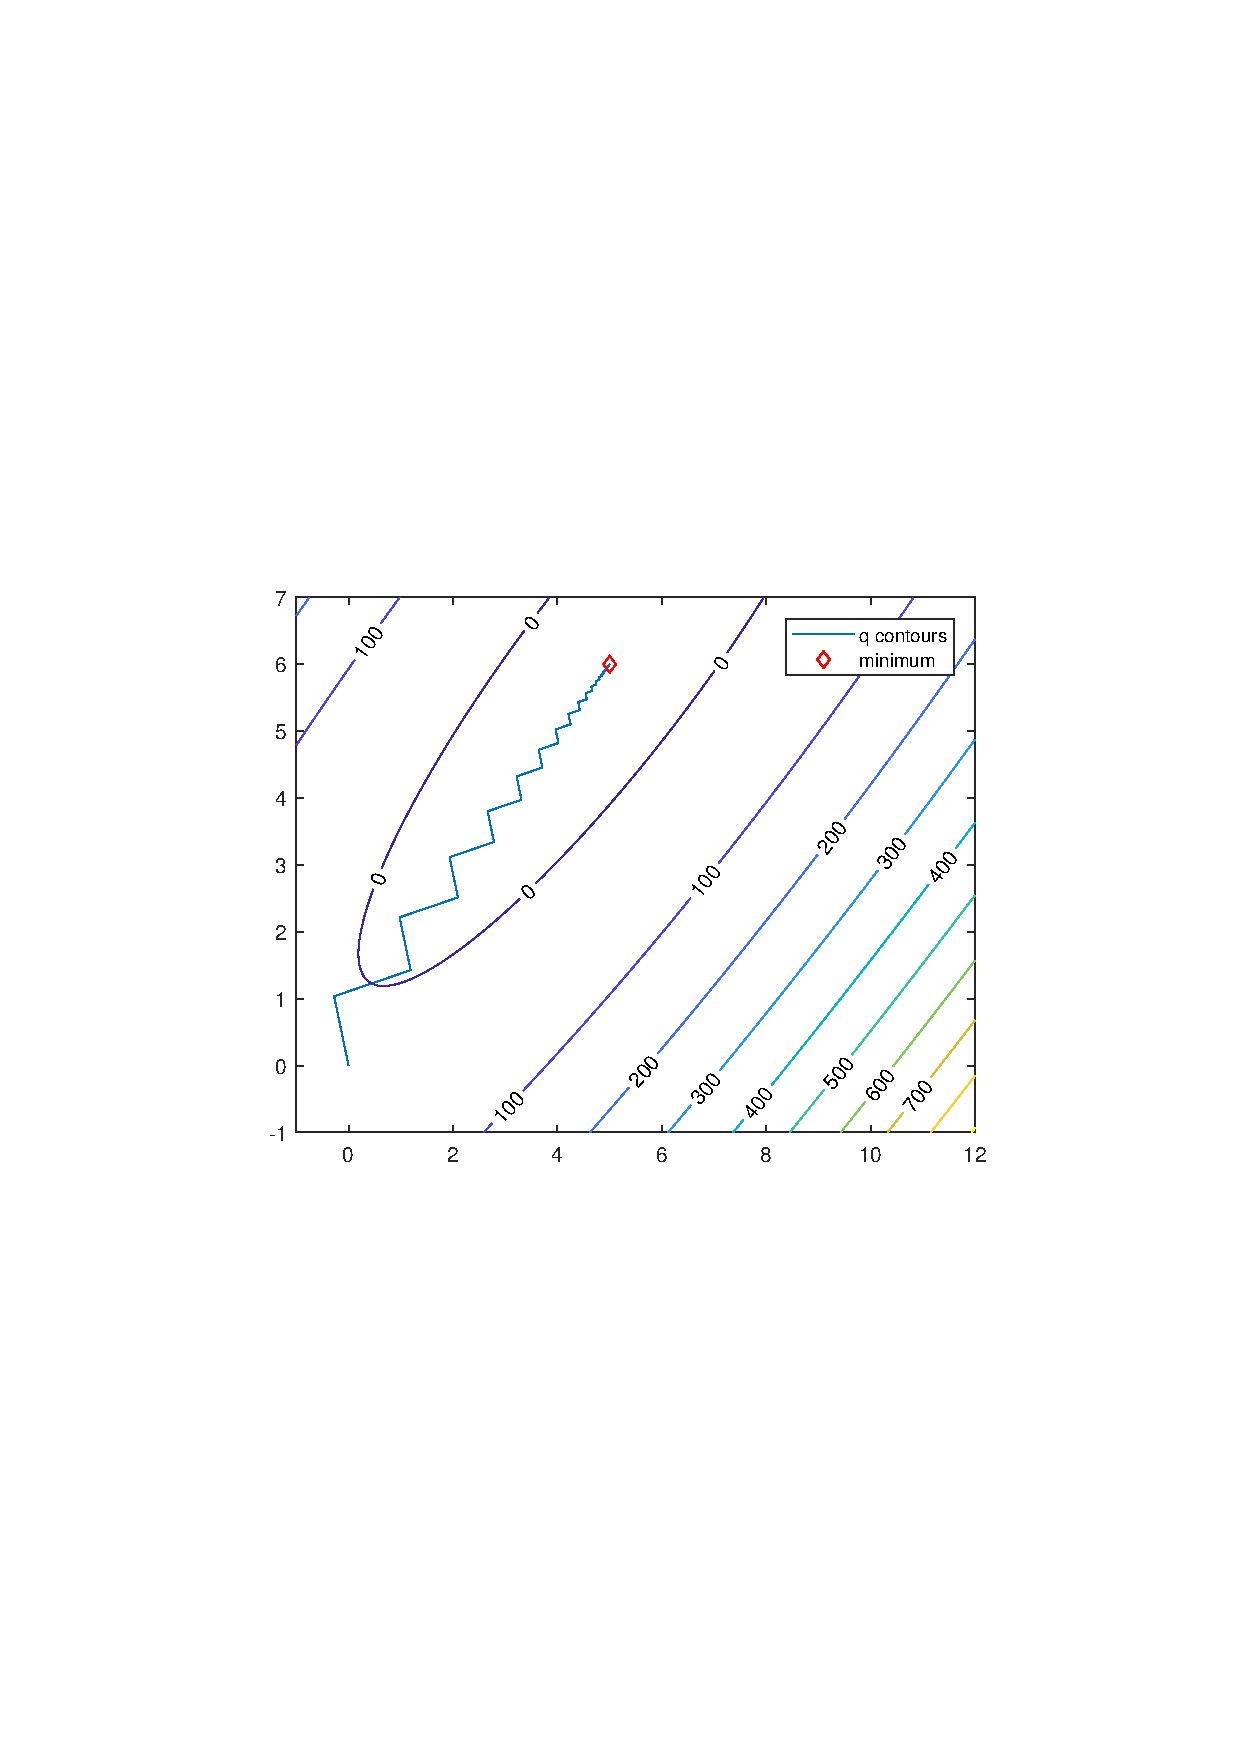
\includegraphics[width=5.7cm]{fig/1_1a.pdf}}
\subfigure{
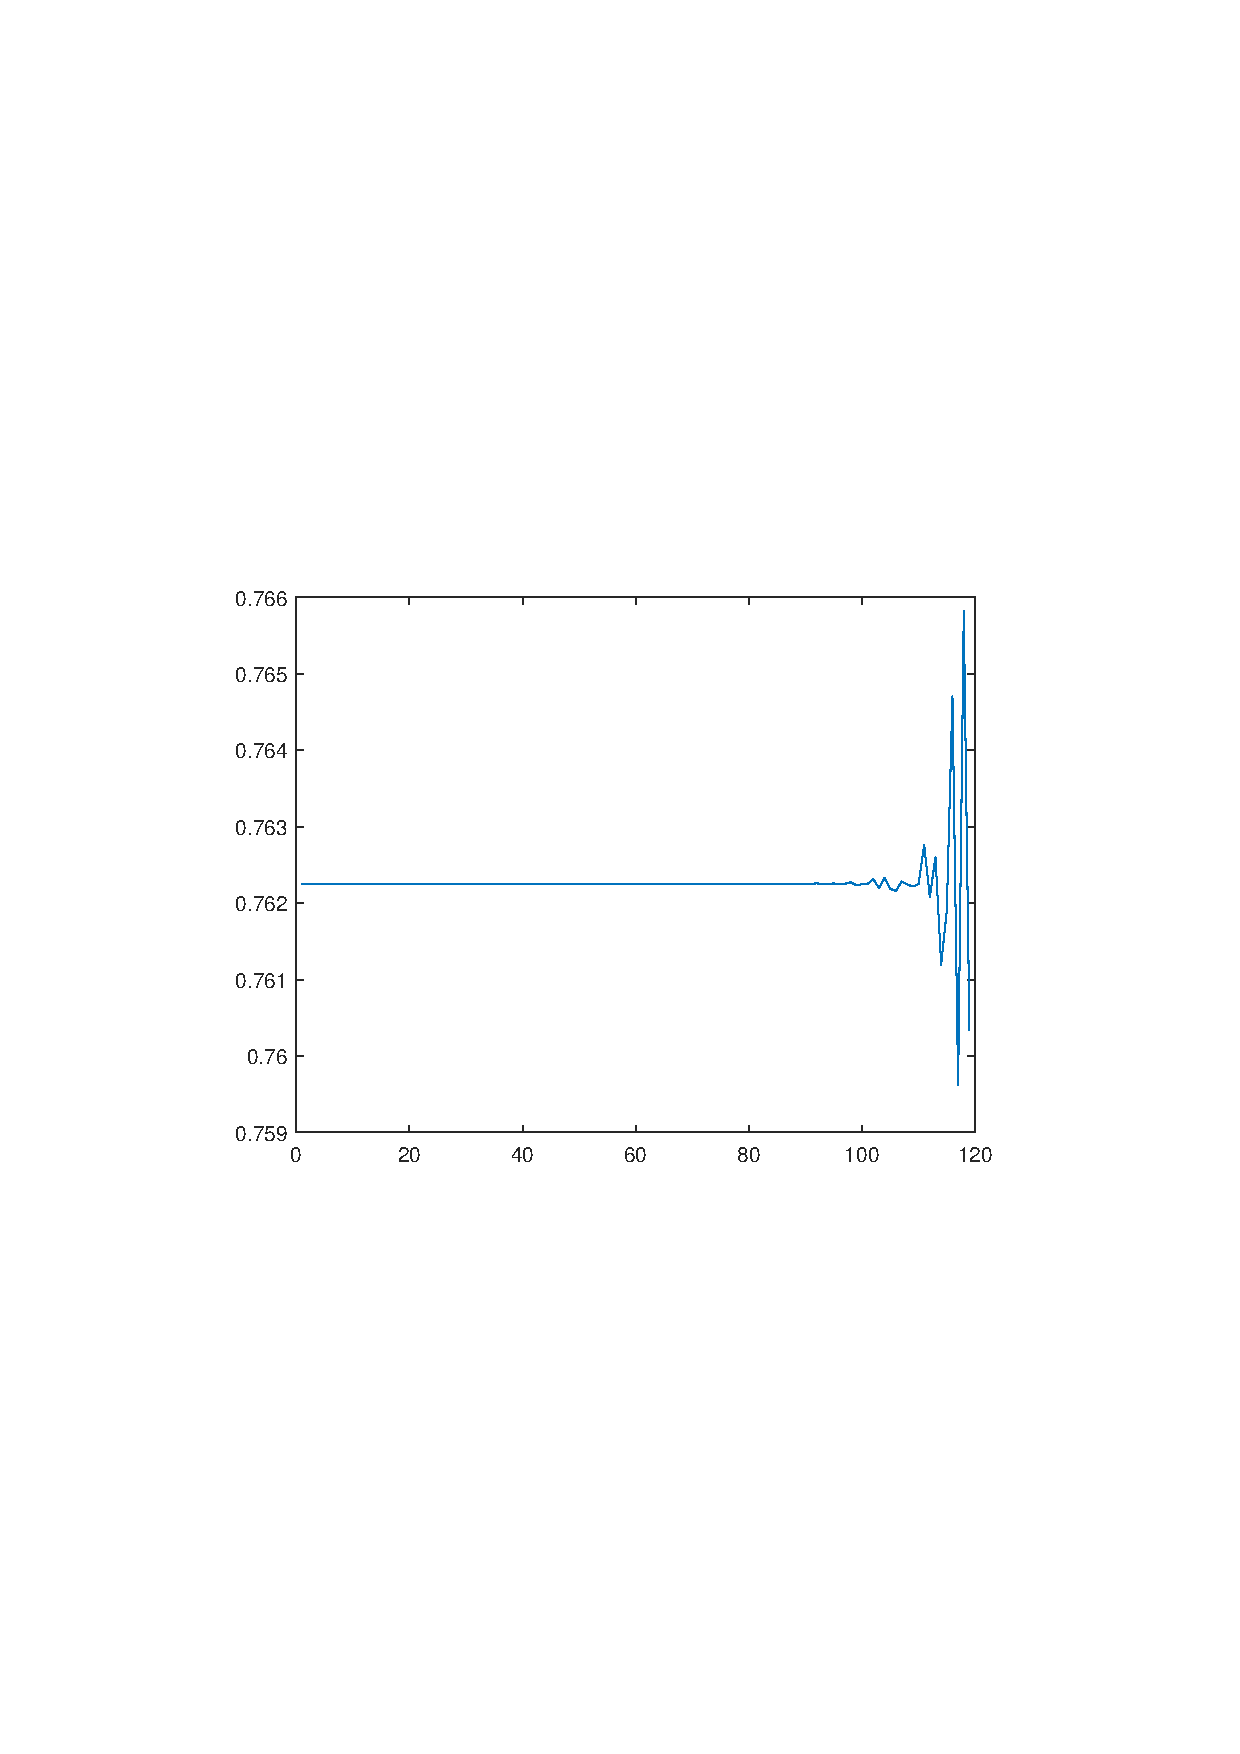
\includegraphics[width=6cm]{fig/1_1b.pdf}}
\caption{Steepest-denscent in (0,0)}
\label{Fig.lable}
\end{figure}

\begin{figure}[H]
\centering
\subfigure{
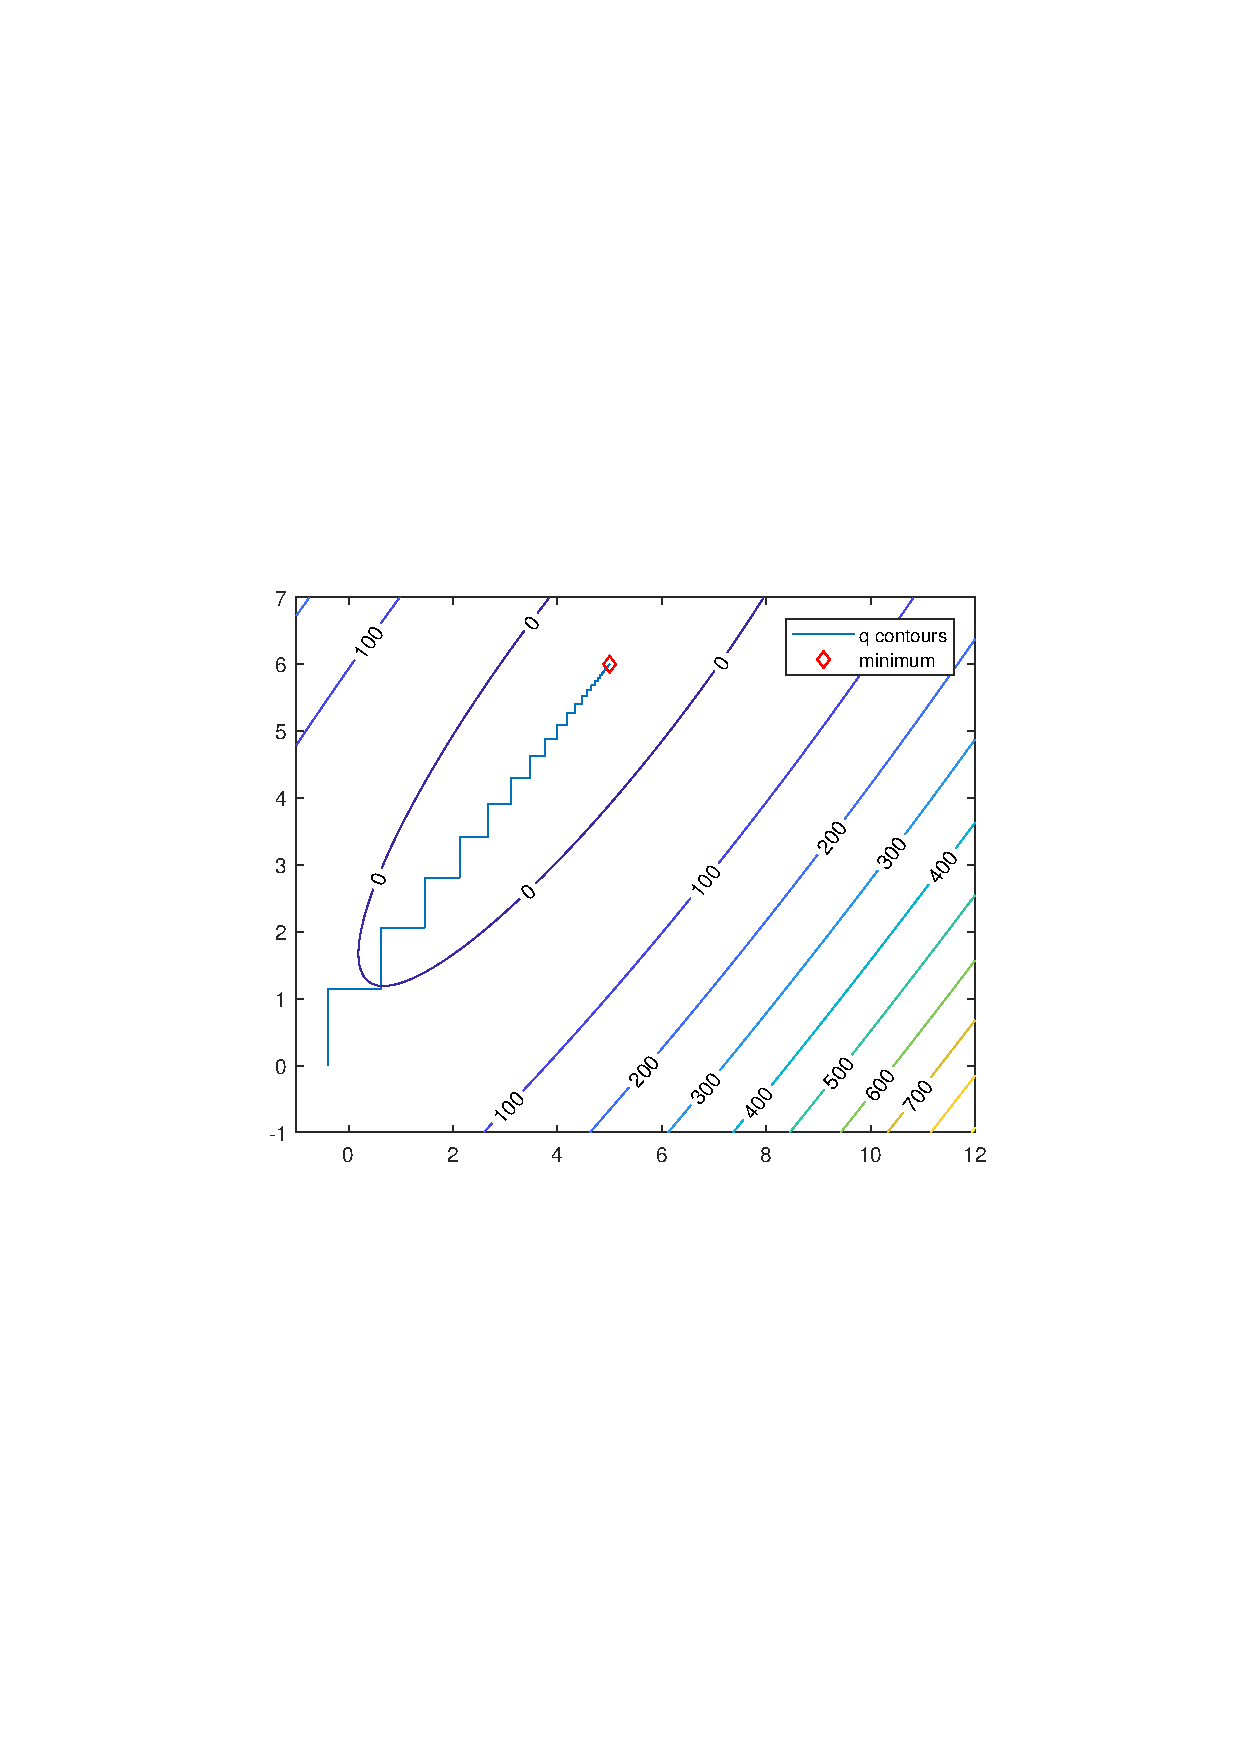
\includegraphics[width=5.7cm]{fig/1_2a.pdf}}
\subfigure{
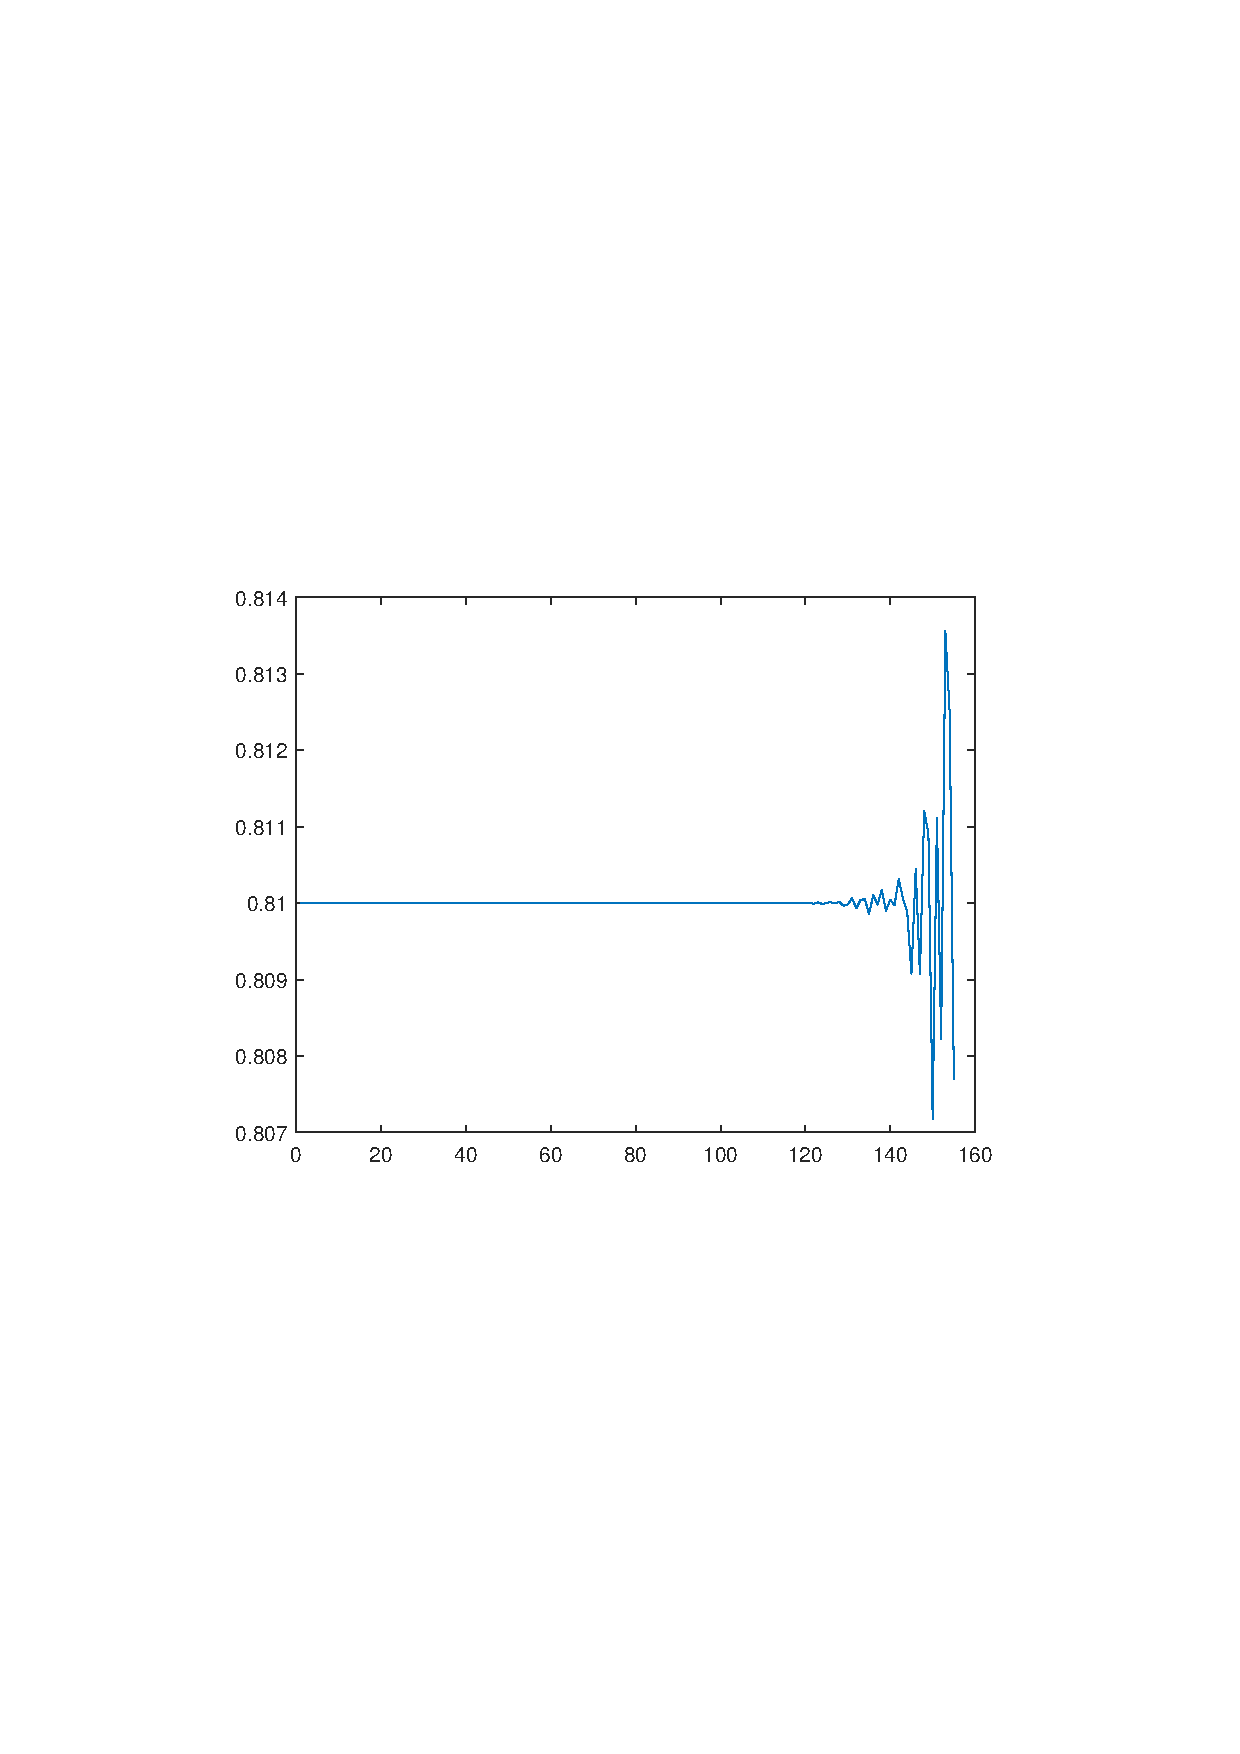
\includegraphics[width=6cm]{fig/1_2b.pdf}}
\caption{Steepest-denscent in (-0.4,0)}
\label{Fig.lable}
\end{figure}

\begin{figure}[H]
\centering
\subfigure{
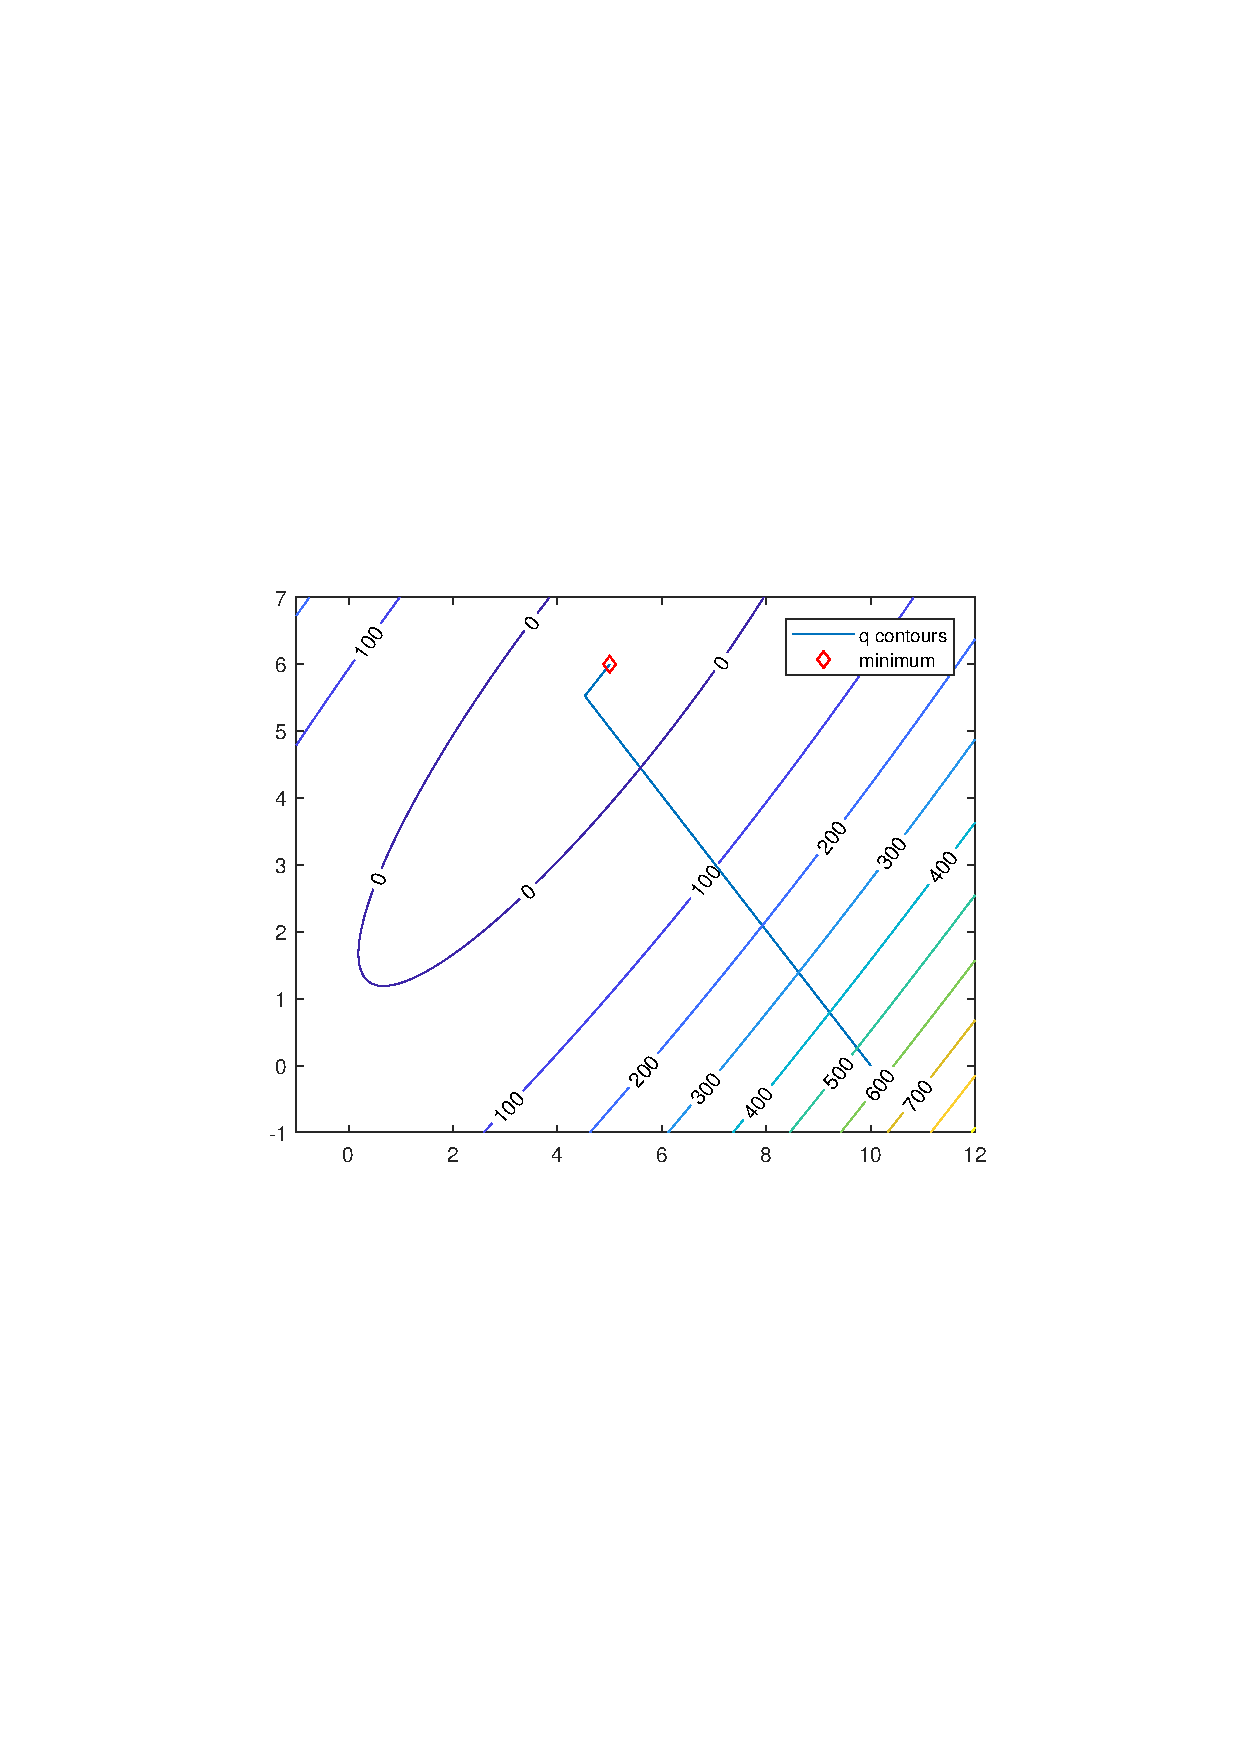
\includegraphics[width=5.7cm]{fig/1_3a.pdf}}
\subfigure{
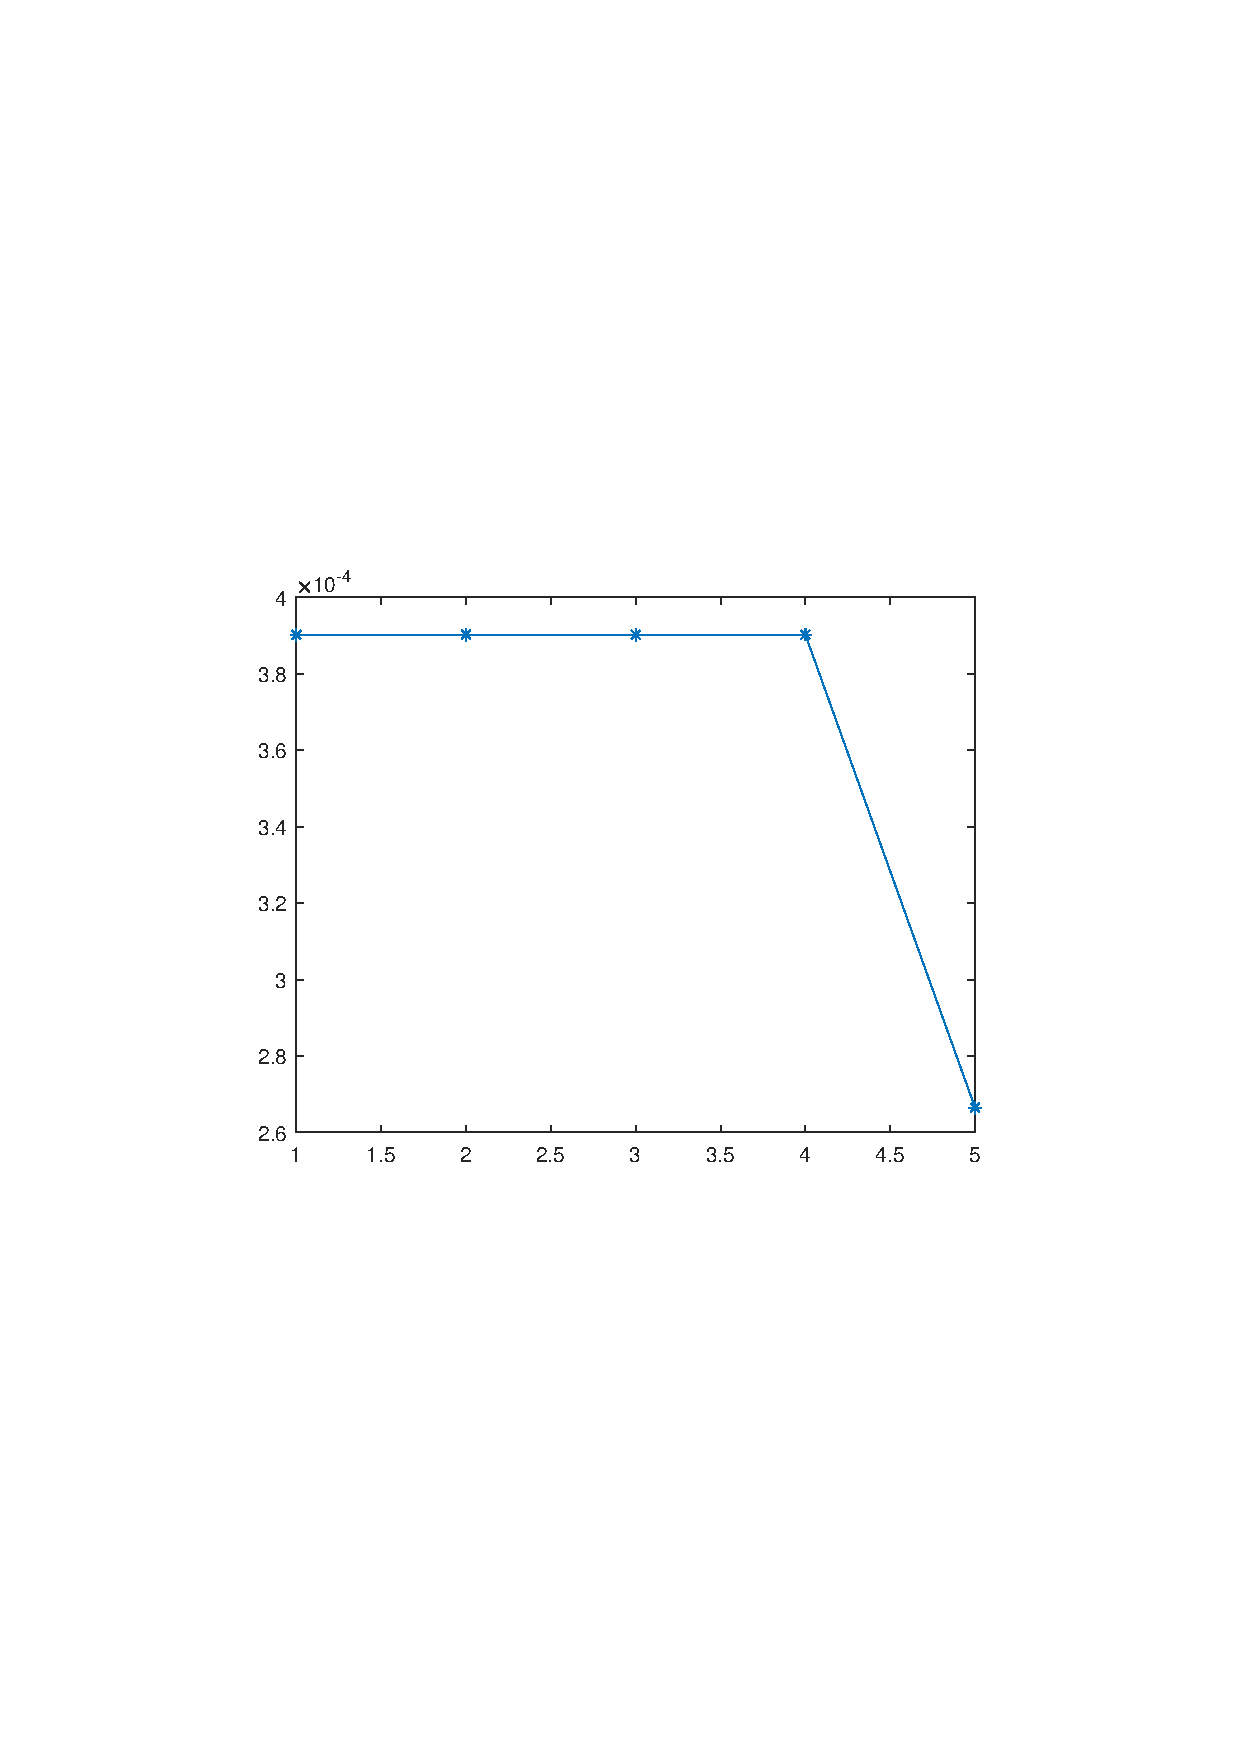
\includegraphics[width=5.8cm]{fig/1_3b.pdf}}
\caption{Steepest-denscent in (10,0)}
\label{Fig.lable}
\end{figure}

\begin{figure}[H]
\centering
\subfigure{
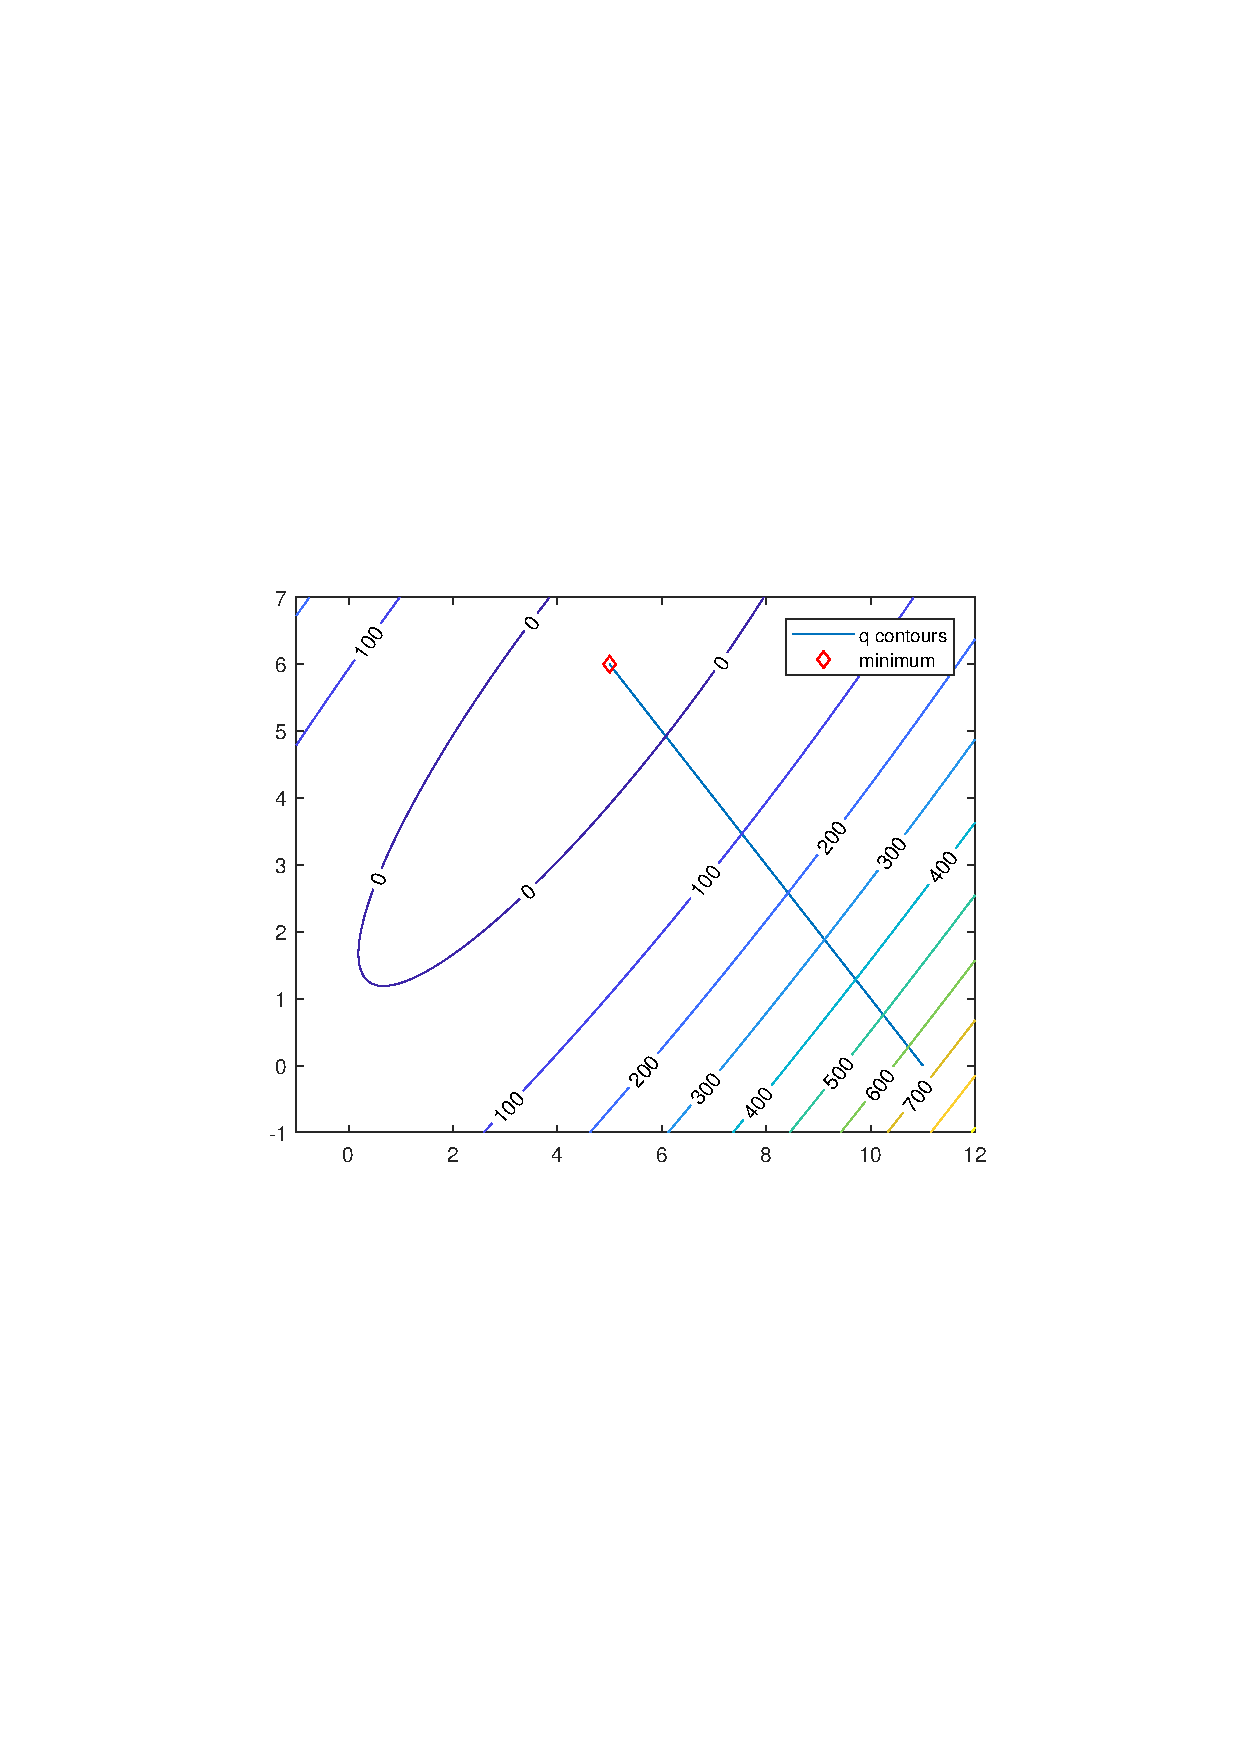
\includegraphics[width=5.8cm]{fig/1_4a.pdf}}
\subfigure{
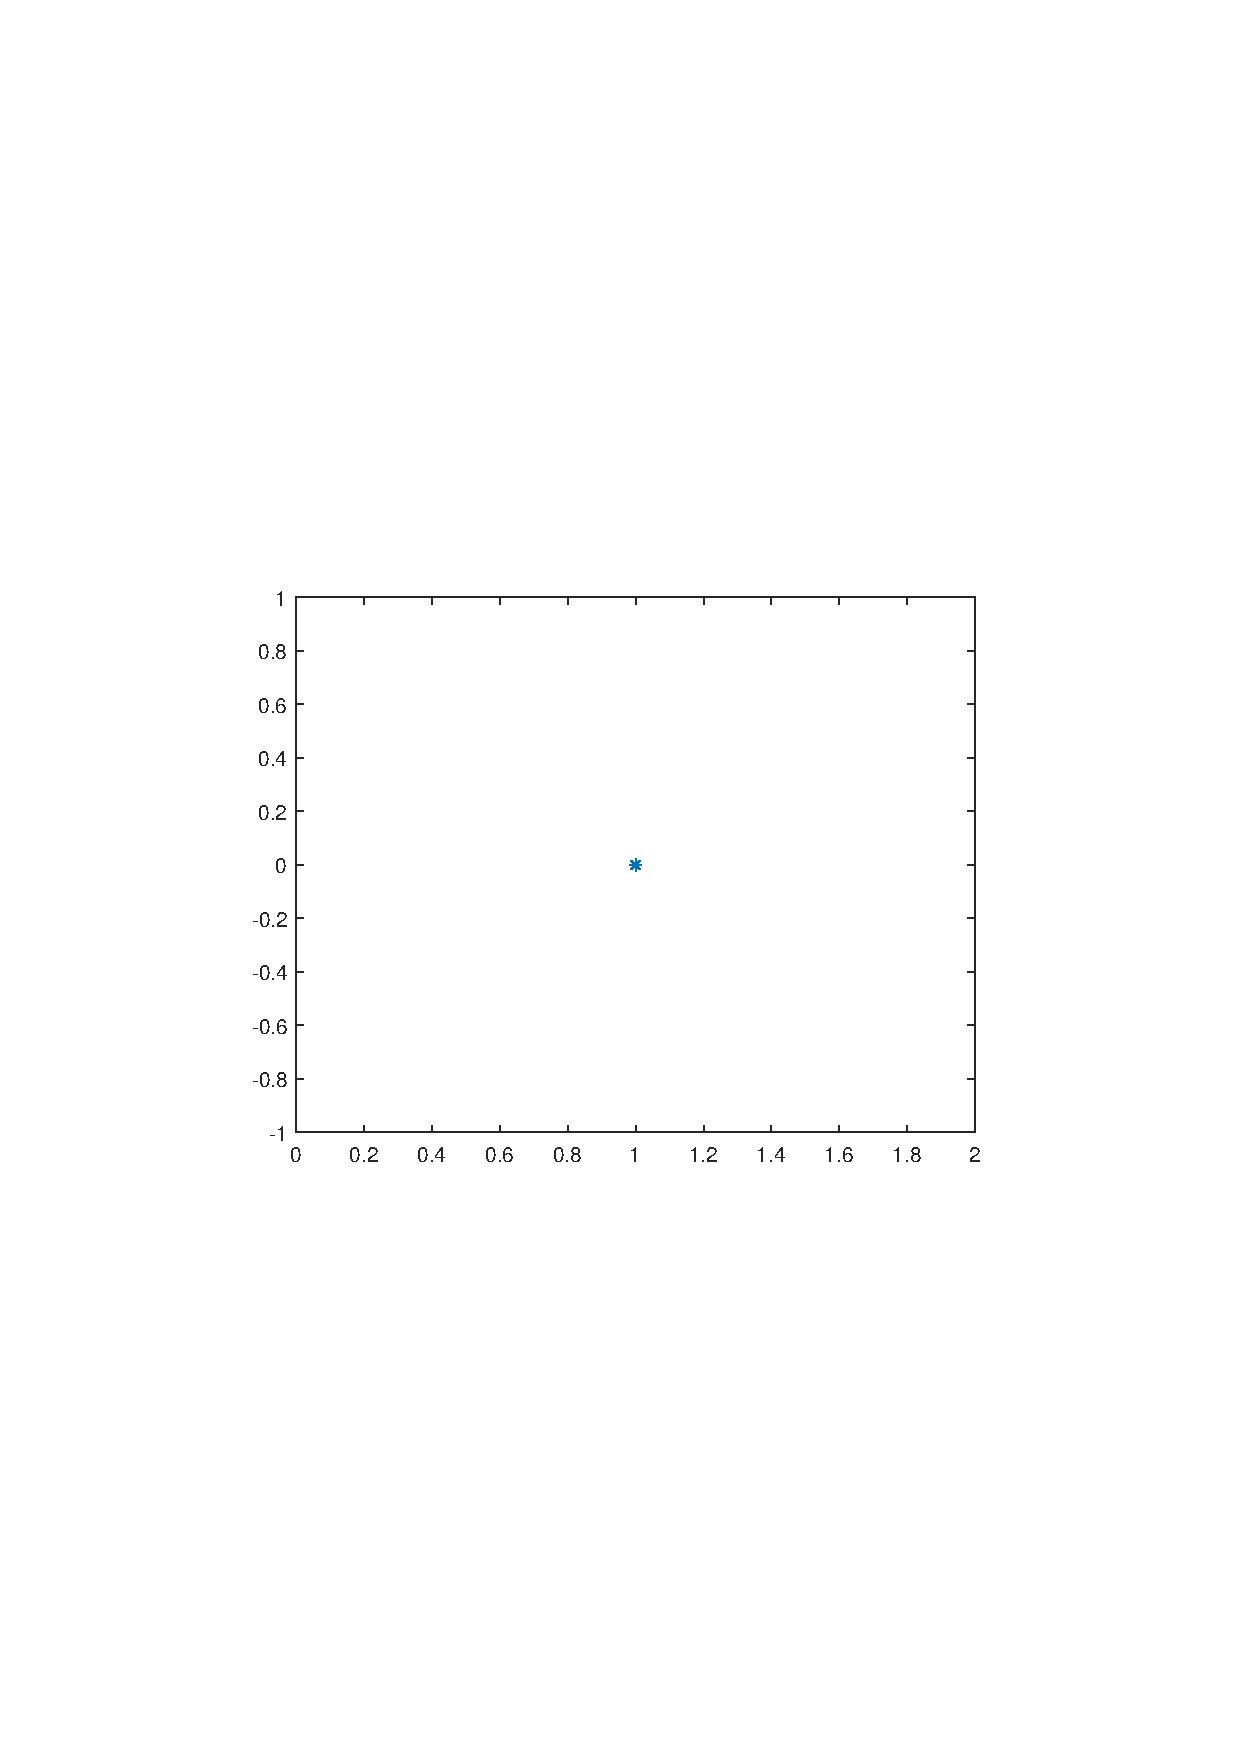
\includegraphics[width=5.9cm]{fig/1_4b.pdf}}

\caption{Steepest-denscent in (11,0)}
\label{Fig.lable}
\end{figure}

\begin{table}[H]
\centering
\caption{收敛因子比较}
	\begin{tabular}{ccccc}
	\toprule
	{起始点}&$(0,0)$&$(-0.4,0)$&$(10,0)$&$(11,0)$\\
	\midrule
	{收敛因子}&0.762255&0.810000&0.000390&0\\
	\bottomrule
	\end{tabular}
\end{table}

\newpage
\subsection{分析}
由于目标函数为凸函数,故使用梯度下降法从这四个不同的起始点出发都能收敛到全局最优点,然而线性收敛因子却互不相同.

由图像可知:在迭代开始后,函数值的收敛速度稳定在一个值左右,直到接近最优点时,收敛速度开始较大幅度波动,估计应该是精度问题导致的。

而且,可以看出,初始点越接近等值线椭圆的狭长端,线性收敛因子越大,在点$(-0.4,0)$处甚至达到了线性收敛因子的上界0.81,而离狭长端越远,收敛因子越小。
这是由于梯度下降在构造搜索方向时没有充分利用到函数的二阶导数信息,在面临“峡谷”状的函数时,会反复震荡到“峡谷”的另一端,而不能直接向最优值方向前进。

求得$G$的特征向量为$(1,1),(-1,1)$,这代表了等值线椭圆的长轴方向和短轴方向,即对于通过最优点$(5,6)$的斜率为1和-1的两条直线,这两条直线上的点都只需一步就能迭代到最优点,$(11,0)=(5,6)-6\times(-1,1)$即是这样一个点。

\begin{figure}[H]
\centering
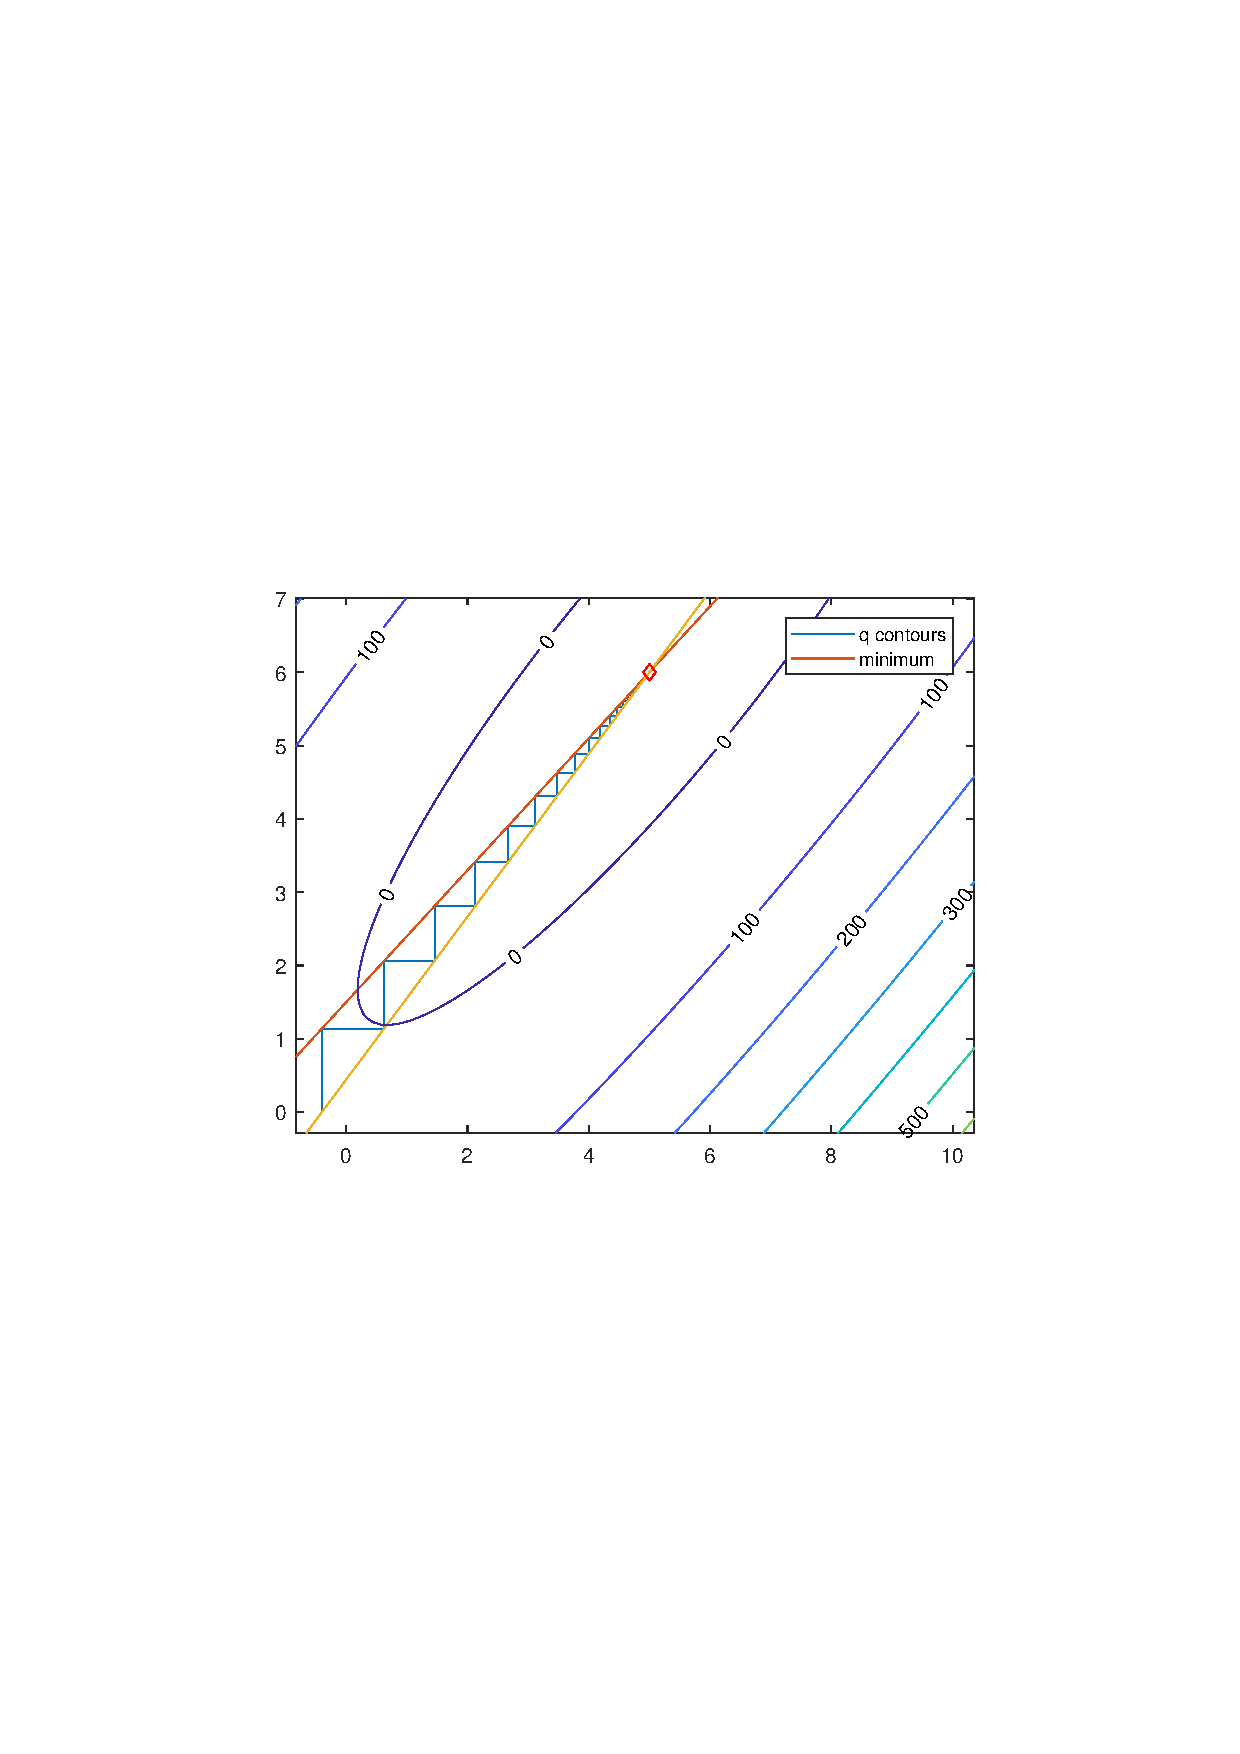
\includegraphics[width=11cm]{fig/1_6.pdf}
\end{figure}

\newpage
然后,我发现对于通过最优点$(5,6)$的斜率为10/9和9/10的两条直线,这两条直线上的点迭代时,收敛速度最慢,能达到线性收敛因子的上界0.81,其中$(-0.4,0)=(5,6)-0.6\times(9,10)$即是这样一个点,但是为什么会是这两条直线呢?我经过非常非常艰苦的探察,最后终于发现了其中的奥妙:

\begin{figure}[H]
\centering
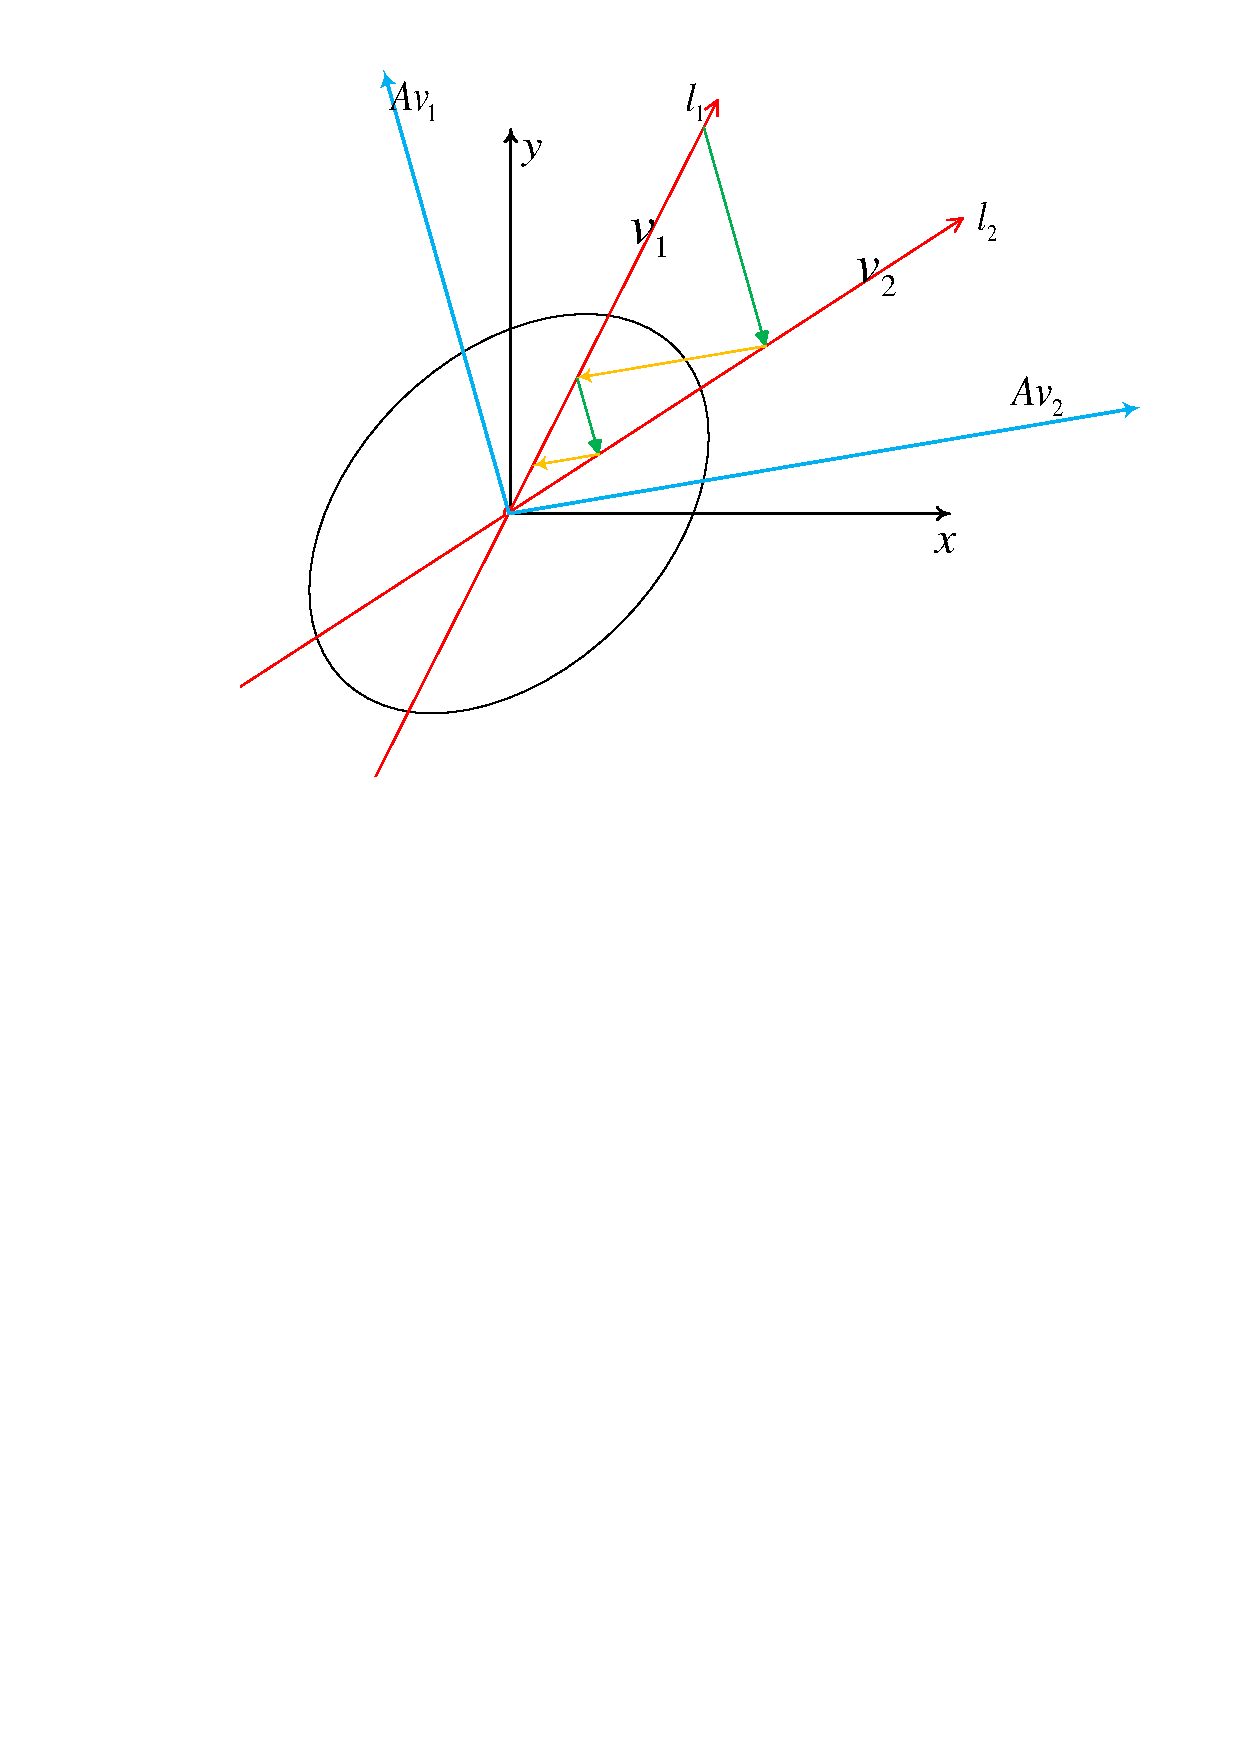
\includegraphics[width=9cm]{fig/1_5.pdf}
\caption{绘制的草图}
\end{figure}

由于一次项只是椭圆位置上的平移,不影响分析,所以不妨去掉一次项和常数项,假设目标函数为
\[f(x)=\dfrac{1}{2}x^TAx,\quad \nabla f(x)=Ax\]

假如有两条向量$v_1,v_2$满足$Av_1\bot Av_2$,其所在直线分别为$l_1,l_2$

对于任意$x^{(k)}\in l_1$,有$x^{(k)}//v_1,\ \nabla f(x^{(k)})=Ax^{(k)}$,因此$x^{(k+1)}$在以$x^{(k)}$为起点沿$Ax^{(k)}$方向的直线上

最速下降法要满足的要求是$\nabla f(x^{(k+1)})\bot Ax^{(k)}$,由于$Av_1\bot Av_2$,故$l_2$上的点$s$都满足$\nabla f(s)=As//Av_2\bot Ax^{(k)}$,又由于解的唯一性,故直线$x^{(k)}+\alpha Ax^{(k)}$与直线$l_2$的交点即为迭代点$x^{(k+1)}$,同理,下一次迭代点也会在$l_1$上,从此以后的点都在这两条直线上反复迭代。并且迭代方向都与$Av_1,Av_2$平行.

至此,我算是明白了最速下降法出现“锯齿”的真正原因,容我细细道来如下:

左乘$A$变化是将空间中所有的向量朝对应特征值按模最大的那个特征向量变换,以这道题为例,这个矩阵有两个特征值19和1,其中19对应的特征向量为$(-1,1)$,1对应的特征向量为$(1,1)$,因此$v_1$向量逆时针旋转来靠拢$(-1,1)$,因为中间夹着另一个特征向量,所以$v_1$向量只能顺时针旋转来靠拢特征向量$(-1,1)$,这是左乘$A$变化.

那么,对于左乘$A^{-1}$变化,其意味着将空间中所有的向量朝对应特征值按模最小的那个特征向量旋转,即$(1,1)$,在这个例子中,对于两个相互垂直的向量$Av_1=(0,19)^T,Av_2=(19,0)^T$,经过左乘$A^{-1}$变化,变成了$v_1=(9,10)^T,v_2=(10,9)^T$,而一般来说,椭圆的长轴对应的特征向量是特征值较小的那一个,因此左乘$A^{-1}$变化将会使向量朝椭圆长轴旋转,而且矩阵$A$的条件数越大,旋转的程度更剧烈,$l_1,l_2$会靠得更接近,直到完全与椭圆长轴重合,而由于每次迭代方向都是固定平行$Av_1,Av_2$的,所以$l_1,l_2$靠得越拢,所需要的迭代次数越多,即收敛速度越小。

那么,什么情况下收敛速度达到最慢呢?我们仔细观察可以发现,由于每一步的步长都投影在$Av_1,Av_2$上,所以总步长是个定值——等于初始点到直线$Av_1,Av_2$的距离之和,显然,当$Av_2$越靠近椭圆长轴,由于$l_2$夹在长轴和$Av_2$之间,所以点在$l_2$上迭代一次的步长越大,对$Av_1$也是如此,所以,只有当$Av_1,Av_2$都离长轴较远时,每一次在$l_1,l_2$上迭代的步长都较小,总步长固定,步长越小,所需要的迭代次数越多。而$Av_1,Av_2$是相互垂直的,所以当$Av_1,Av_2$的角平分线与椭圆长轴重合时,迭代次数最多。

在这个例子中,由于椭圆长轴对应的特征向量是$(1,1)$,因此不难看出$Av_1,Av_2$应该分别和y轴、x轴重合,此时每一次迭代也都平行y轴、x轴.

据此,我们还能在这种情况下进行收敛性的分析:根据三角形相似,可以算出步长$a_{k+2}/a_k=\tan^2(\pi/4-\theta)$,其中$\theta$为$l_1$与椭圆长轴的夹角,同时根据矩阵的坐标变换,可知$tan(\theta)=\dfrac{\lambda_1}{\lambda_2}$,其中$\lambda_1$是最大特征值,$\lambda_2$是最小特征值,那么可以算出$a_{k+2}/a_k=\tan^2(\pi/4-\theta)=(\dfrac{1-tan(\theta)}{1+tan(\theta)})^2$,继续由三角形相似可以得到$a_{k+1}/a_k=a_{k+2}/a_{k+1}=\dfrac{1-tan\theta}{1+tan\theta}$,由于函数值与步长成二次关系,故\[\dfrac{f(k+1)}{f(x)}=(\dfrac{1-tan\theta}{1+tan\theta})^2=(\dfrac{1-\lambda_1/\lambda_2}{1+\lambda_1/\lambda_2})^2\]



